% Gemini theme
% https://github.com/anishathalye/gemini

\documentclass[20pt, final]{beamer}

% ====================
% Packages
% ====================

%\usepackage[T1]{fontenc}
\usepackage{lmodern}
\usepackage[size=a1, scale=1.0]{beamerposter}
\usetheme{gemini}
\usecolortheme{gemini}
\setbeamerfont{block body}{family=\Lato,size={\fontsize{25}{27}}}
\setbeamerfont{enumerate item}{size={\fontsize{25}{27}}}

\usepackage{graphicx}
\usepackage{booktabs}
\usepackage{tikz}
\usepackage{pgfplots}
\definecolor{amethyst}{rgb}{0.6, 0.33, 0.73}
\usepackage{fontawesome}
\pgfplotsset{compat=1.14}
\usepackage{anyfontsize}

\usepackage{tcolorbox}

\usepackage{wrapfig}
\usepackage{braket}
\usepackage{bm}


%% ---------- useful for the schema ---------

\usetikzlibrary{positioning,arrows,calc,math,angles,quotes}
\usetikzlibrary{arrows,automata}
\usetikzlibrary{positioning}
\usetikzlibrary{arrows.meta,
                bending,
                intersections,
                quotes,
                shapes.geometric}

\tikzset{
    state/.style={
           rectangle,
           rounded corners,
           draw=black, very thick,
           minimum height=1em,
           inner sep=2pt,
           text centered,
           },
}



\definecolor{darkmidnightblue}{rgb}{0.0, 0.2, 0.4}

% ====================
% Lengths
% ====================

% If you have N columns, choose \sepwidth and \colwidth such that
% (N+1)*\sepwidth + N*\colwidth = \paperwidth
\newlength{\sepwidth}
\newlength{\colwidth}
\setlength{\sepwidth}{0.025\paperwidth}
\setlength{\colwidth}{0.3\paperwidth}


% useful for the logos

\logoright{
\includegraphics[height=4cm]{figures/qibolab_paper_qr.png}}
\logoleft{
\includegraphics[height=4cm]{figures/qibo_qr.png}}


\newcommand{\separatorcolumn}{\begin{column}{\sepwidth}\end{column}}

% ====================
% Title
% ====================

\title{\texttt{qibo}: a full-stack framework for simulation, control
and calibration of self-hosted qubit devices}

\author{Stefano Carrazza\inst{1  }\inst{2  }\inst{3  }}

\institute[shortinst]{
  \inst{1  } TIF Lab, Dipartimento di Fisica, Universit\`a degli Studi
  di Milano, Milan, Italy. 
  \samelineand 
  \inst{2  } CERN, Theoretical Physics Department, CH-1211
  Geneva 23, Switzerland.
  \samelineand
  \inst{3  } Quantum Research Center, Technology Innovation Institute, Abu Dhabi, UAE.
  }

% ====================
% Footer (optional)
% ====================

\footercontent{
}
% (can be left out to remove footer)

% ====================
% Logo (optional)
% ====================

% use this to include logos on the left and/or right side of the header:
% \logoright{\includegraphics[height=7cm]{logo1.pdf}}
% \logoleft{\includegraphics[height=7cm]{logo2.pdf}}

% ====================
% Body
% ====================

\begin{document}

\begin{frame}[t]
\begin{columns}[t]
\separatorcolumn

\begin{column}{\colwidth}

  % abstract
  \begin{block}{Abstract}
    We present \texttt{qibo}~\cite{Efthymiou_2021}, a full-stack and open source framework which can be 
    used for:
    
    \begin{itemize}
      \item[\faCode] efficiently simulate quantum computation routines, both in 
      circuit notation and in the context of adiabatic computation;
      \item[\faCogs] control self-hosted quantum devices with an hardware-agnostic
      approach;
      \item[\faPencil] performing quantum characterization, calibration and 
      verification routines on the hosted qubits.
    \end{itemize}
  
  \end{block}

  % qibo ecosystem
  \begin{block}{\texttt{OVERVIEW:} the \texttt{qibo} ecosystem}
  \begin{figure}
    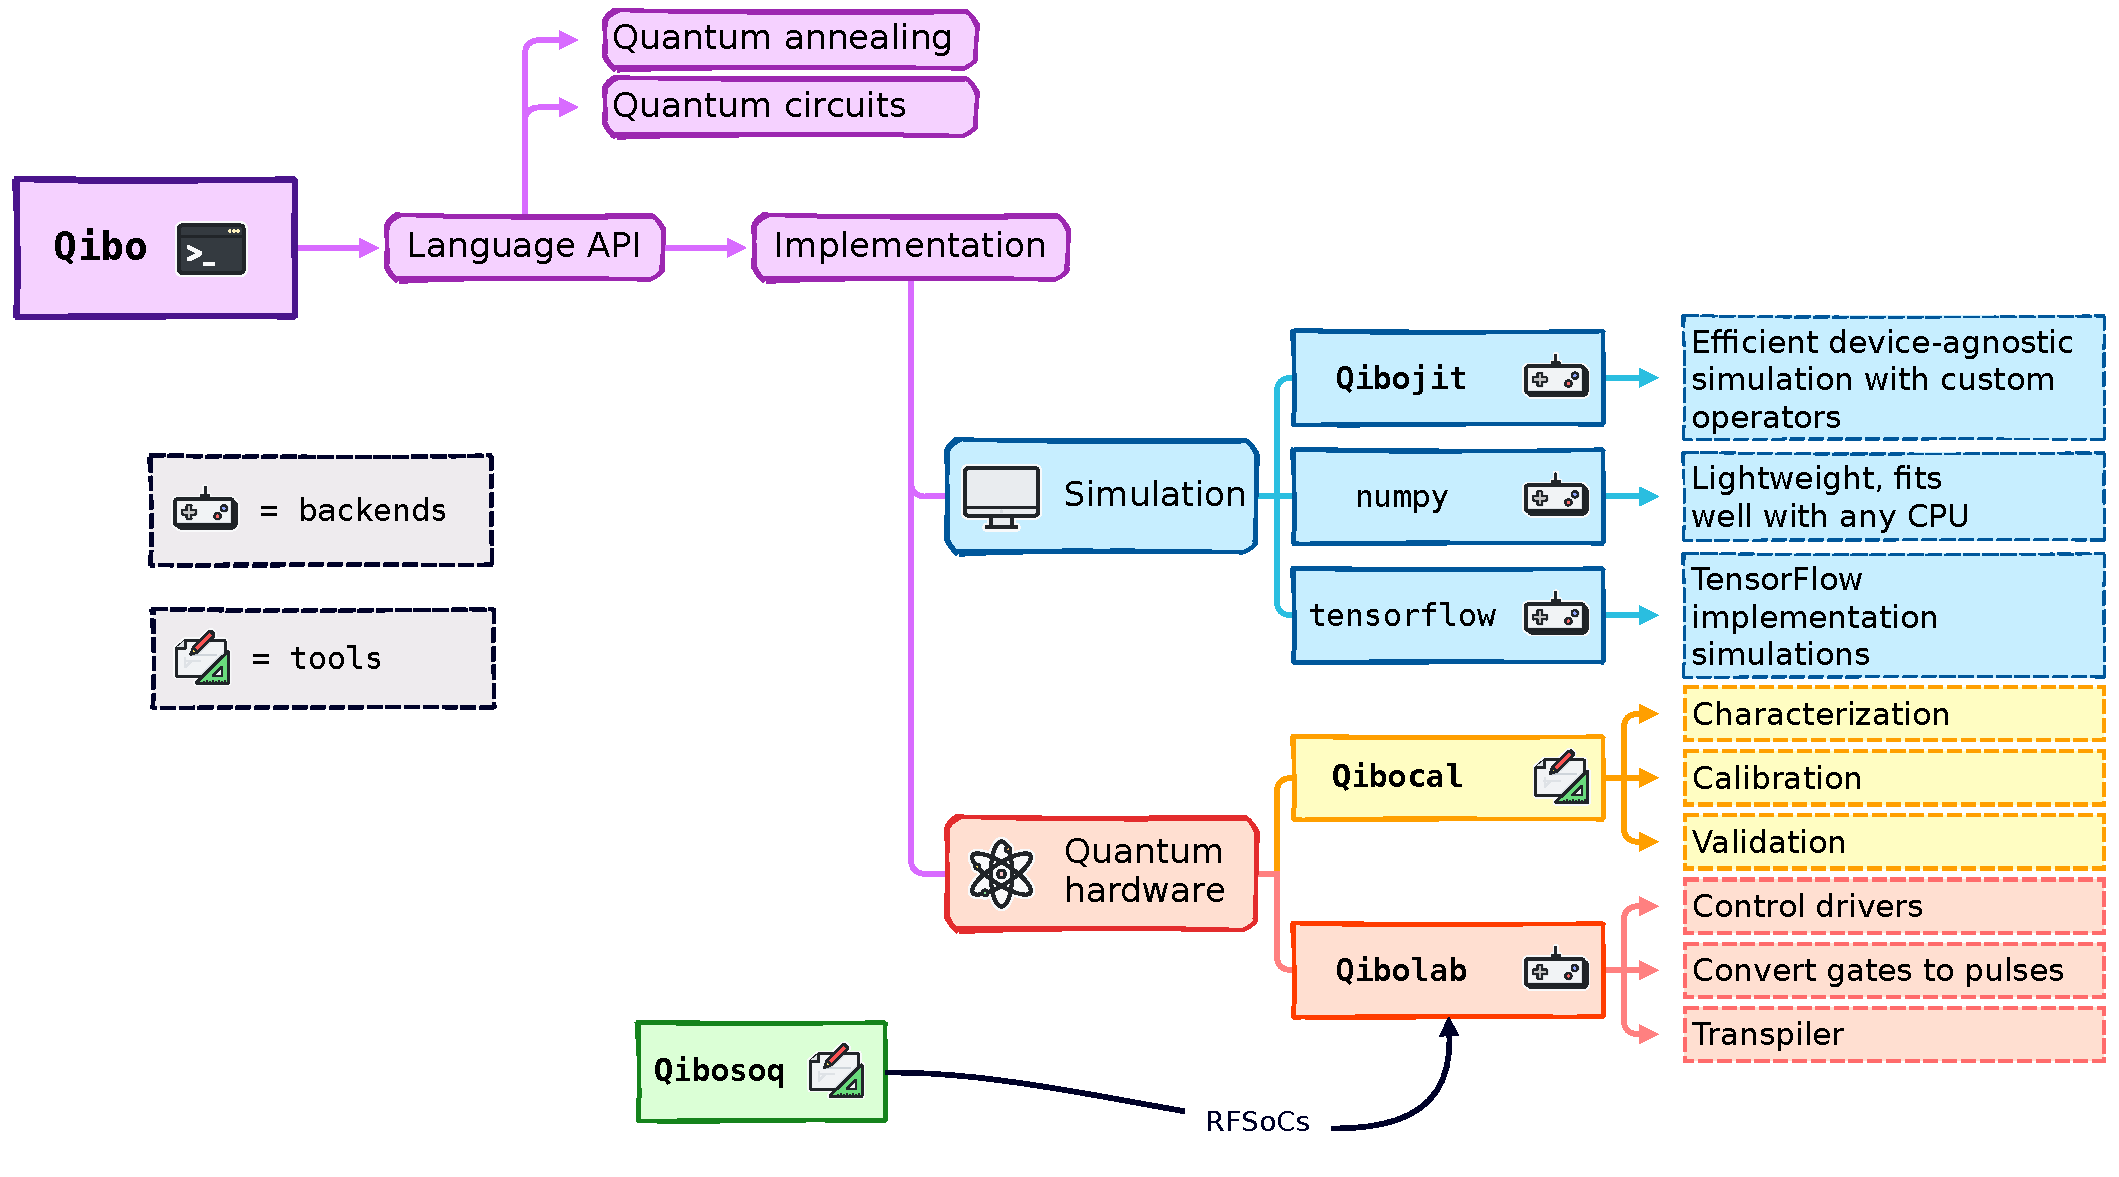
\includegraphics[width=1  \textwidth]{figures/qibo_ecosystem.pdf}
  \end{figure}
  \end{block}

  % simulation - qibojit
  \begin{block}{\texttt{SIMULATION:} \texttt{qibojit}}
  We do state vector simulation of a system of qubits $\{\sigma_j\}$, 
  which solves:
  \begin{equation}
  \psi'(\sigma_1, ..., \sigma_n) = \sum_{\tau'}G(\tau, \tau') \psi(\sigma_1, ..., 
  \tau', ..., \sigma_n),
  \end{equation}
  The number of operations scales exponentially with $N_{\rm qubits}$, thus we 
  built the \texttt{qibojit} backend~\cite{Efthymiou_2022}.

  \begin{figure}
    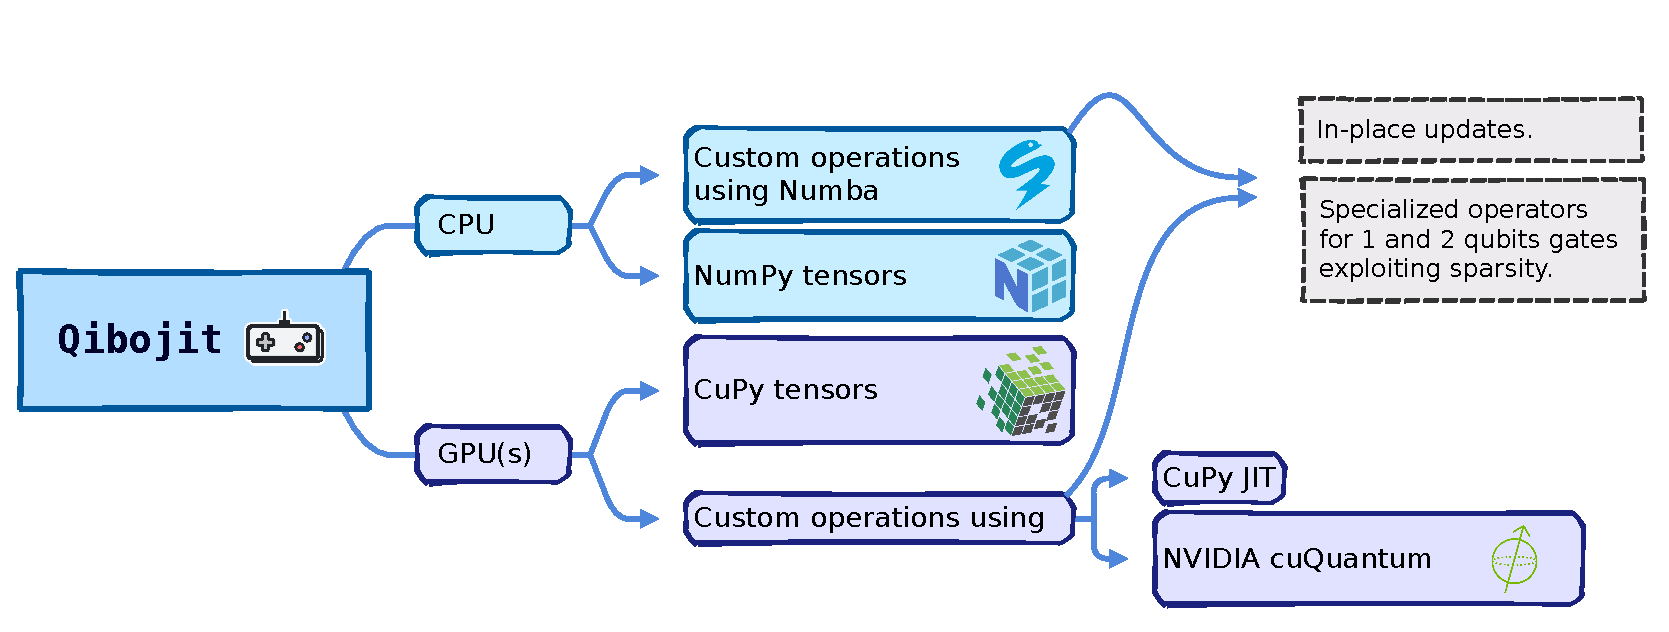
\includegraphics[width=1  \textwidth]{figures/qibojit.pdf}
  \end{figure}
  \end{block}

\end{column}

  \separatorcolumn

\begin{column}{\colwidth}

  % simulation - annealing
  \begin{block}{\texttt{SIMULATION:} adiabatic computation}
  In \texttt{qibo} symbolic hamiltonians can be defined and used to perform 
  adiabatic computation:
  \begin{equation}
  H_{\rm ad}(\tau; \bm{\theta}) = \bigl[ 1 - s(\tau; \bm{\theta}) \bigr] H_0 +  
  s(\tau; \bm{\theta}) H_1,
  \end{equation}
  even following a parametric scheduling $s(\tau, \bm{\theta})$.


  \begin{tikzpicture}[->,>=stealth']

  
 
  % step j
  \node[
    state, 
    xshift=1cm,
    inner sep=0.75cm,
    fill=amethyst!15,
    label=Step $j$] (j) 
    {
      \begin{tabular}{l}
      $\ket{\psi(\tau_j)}$
      \end{tabular}
    };
  
  % Uj
  \node[
  state, 
  above of=j, 
  xshift=1cm,
  yshift=0.5cm, 
  anchor=center,
  node distance = 4cm,
  inner sep=0.75cm,
  fill=amethyst!15,
  label=Trotter at $\tau_j$] (U)
  {
    \begin{tabular}{l}
    $U_j = \exp \bigl[-iH_j \text{d}\tau\bigr]$ 
    \end{tabular}
  };

    % Solve schrodinger locally
  \node[
  state, 
  right of=j, 
  xshift=1cm,
  yshift=0cm, 
  anchor=center,
  node distance = 9cm,
  inner sep=0.75cm,
  fill=amethyst!15,
  label=Execute circuit] (AE)
  {
    \begin{tabular}{l}
    $\ket{\psi(\tau_{j+1})} = U_j \ket{\psi(\tau_j)}$ 
    \end{tabular}
  };

  \draw[line width=0.8mm] (3.5, 0)  to[out=0, in=180] (5.8, 0);
  \draw[line width=0.8mm] (7, 4.5)  to[out=0, in=90] (11, 2.5);
  \draw[line width=0.8mm] (16.2, -1)  to[out=330, in=235] (-3, 1);
  
  \node[
    draw,
    fill=amethyst!15,
    inner sep=0.5cm,
  ] at (8,-5.5) {$j = j + 1$};

  \end{tikzpicture}
  \end{block}


  \begin{block}{\texttt{CONTROL: qibolab}}
  The full-stack framework is hardware agnostic!
  \begin{figure}
    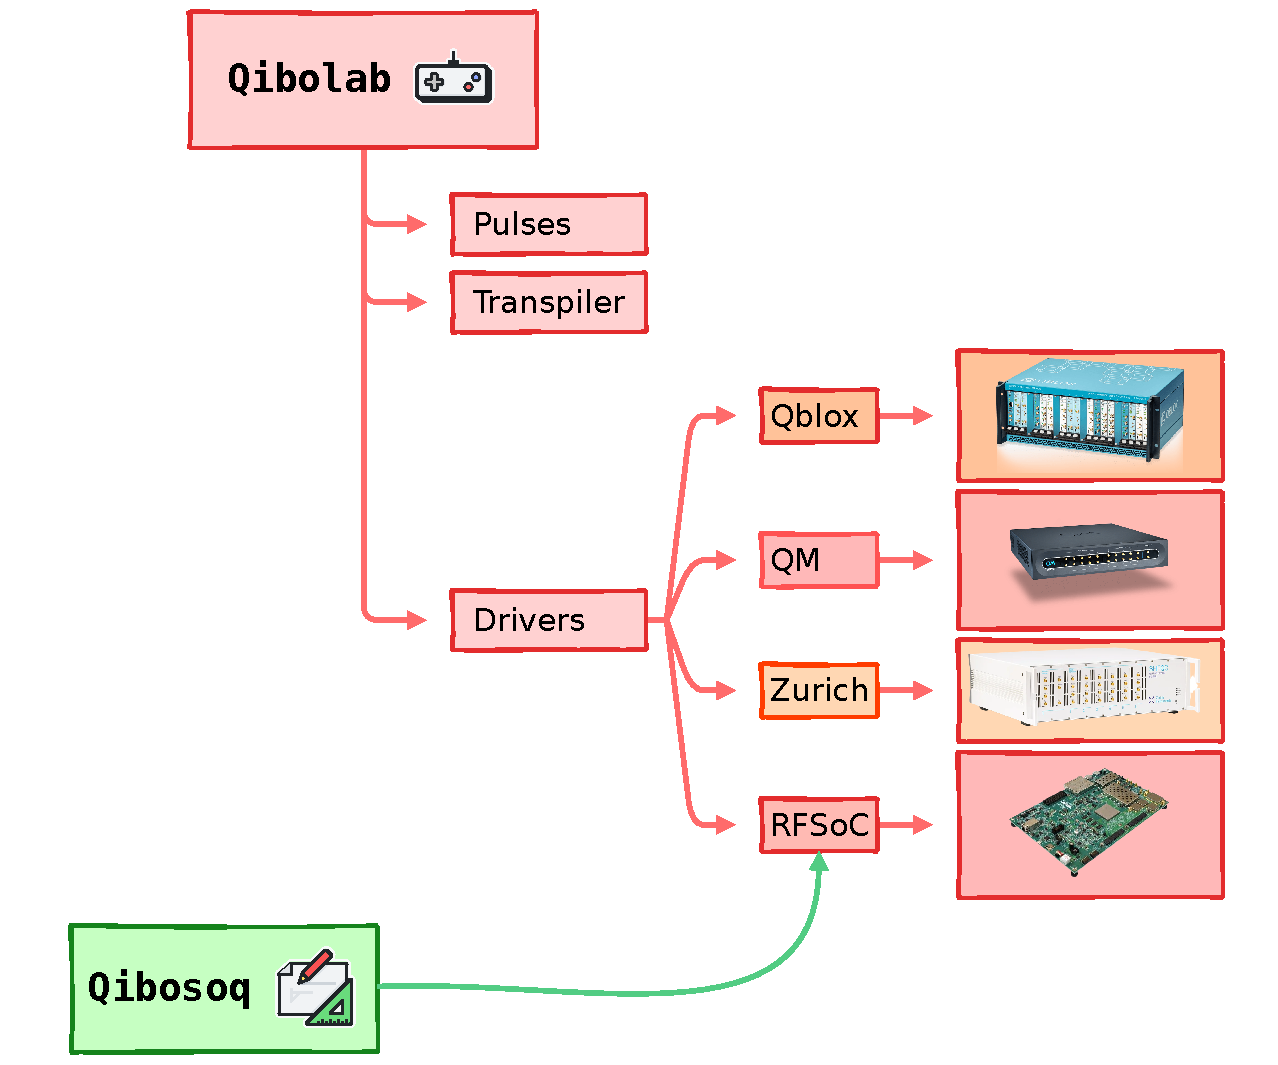
\includegraphics[width=0.7  \textwidth]{figures/qibolab_instruments.pdf}
  \end{figure}

  The \texttt{qibo}'s high level language can be deployed on any quantum hardware
  technology by defining a \texttt{platform} object:
  \begin{enumerate}
  \item a quantum computation algorithm can be written with \texttt{qibo};
  \item define \texttt{custom\_platform} object for a self-hosted device;
  \item the hardware backend can be set via \texttt{qibo.set\_backend('qibolab', 'custom\_platform')}.
  \end{enumerate}
  \end{block}
  \end{column}

  \separatorcolumn

\begin{column}{\colwidth}


  \begin{block}{\texttt{CALIBRATION: qibocal}}
  Each qubit needs characterization, calibration, verification~\cite{pasquale2023opensource}.
  \begin{figure}
    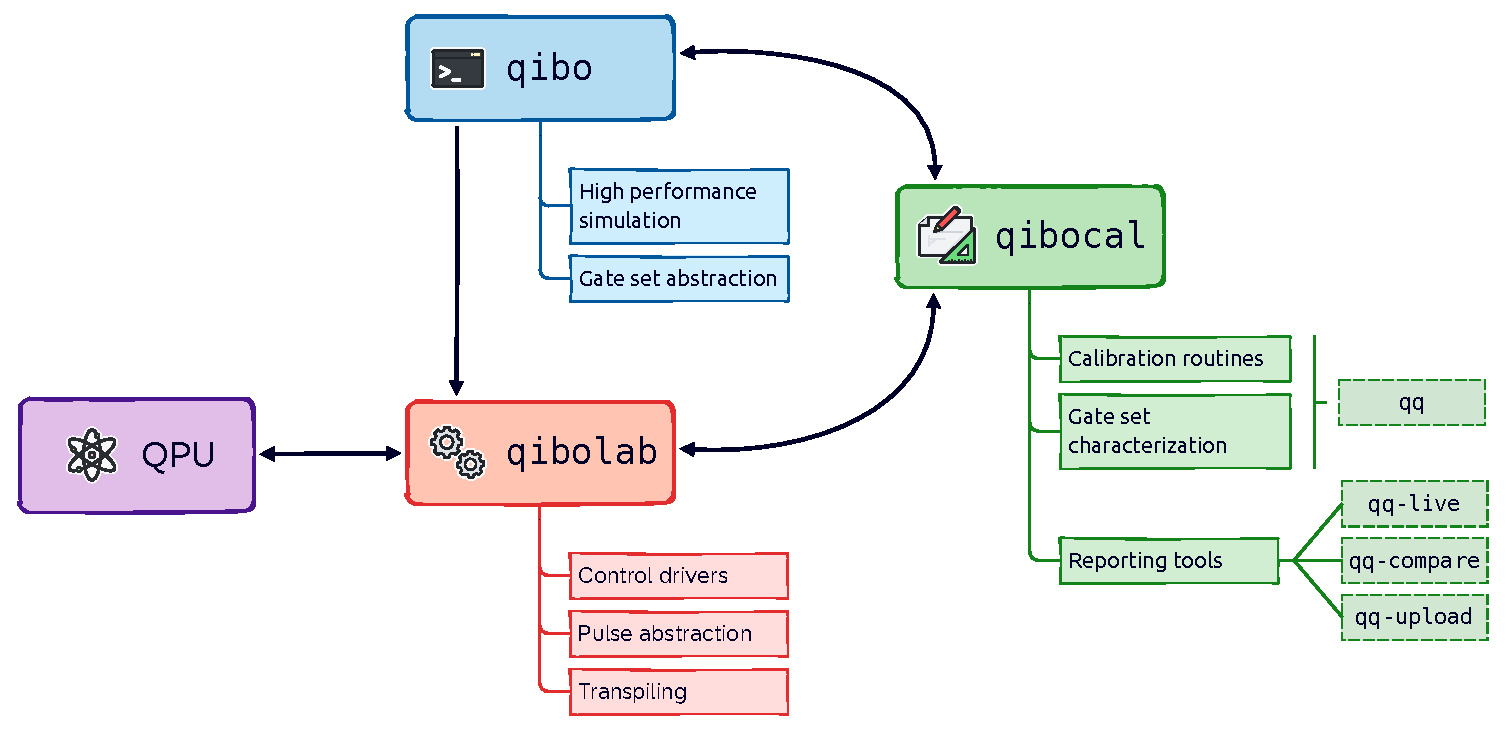
\includegraphics[width=1  \textwidth]{figures/qibocal.pdf}
  \end{figure}
  \end{block}

  \begin{block}{Full-stack gradient descent using \texttt{qibo}}
  We train a quantum circuit to fit the $u$-quark Parton Distribution Function. 
  The full gradient descent
  is performed on the device controlled via RFSoC~\cite{efthymiou2023qibolab}.
  \begin{figure}
    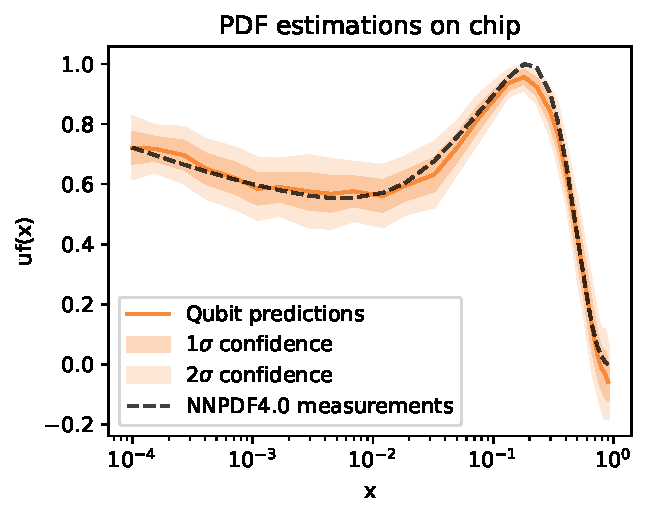
\includegraphics[width=0.8  \textwidth]{figures/qpdf.pdf}
  \end{figure}
  \end{block}

  \begin{block}{References}
  \nocite{*}
    \small {\bibliographystyle{ieeetr}\bibliography{poster.bib}}
  \end{block}

\end{column}

\separatorcolumn
\end{columns}
\end{frame}

\end{document}
